% CS229 Final Paper
\documentclass{article}

\usepackage[final]{cs229}
\usepackage[utf8]{inputenc}
\usepackage[T1]{fontenc}
\usepackage{hyperref}
\usepackage{url}
\usepackage{booktabs}
\usepackage{amsfonts}
\usepackage{nicefrac}
\usepackage{microtype}
\usepackage{xcolor}
\usepackage{amsmath}
\usepackage{fancyhdr}
\usepackage{graphicx}

\pagestyle{fancy}
\fancyhf{}
\fancyhead[C]{CS229 Final Paper}
\renewcommand{\headrulewidth}{0.4pt}

\renewcommand{\maketitle}{
 \begin{center}
  {\bf \large Weight-Space Merging across Medical Imaging Datasets}\\
  \vspace{0.1cm}
  {\bf Sonnet Xu} \quad sonnet@stanford.edu\\
  \vspace{0.2cm}
 \end{center}
}

\begin{document}

\maketitle

\begin{abstract}
Weight-space merging promises multiple specialist capabilities in a single model, but it is unclear how reliably it works for medical imaging, where tasks span nearly disjoint visual domains (radiology, dermoscopy, histopathology). We run a controlled study across up to 7 ViT backbones, 4 medical imaging datasets, 8 merging methods, and 3 seeds, evaluated against an oracle-router upper bound and a multi-task joint-training (MTL) baseline. Three findings. (i) Merge forgetting is overwhelmingly a property of the target dataset, not of the method or the backbone, with per-dataset mean forgetting spanning $0.06$ (radiology) to $0.23$ (dermoscopy) and dataset+method indicators dominating cross-architecture predictability. (ii) Where merging fails most (TCGA, a 9-point gap to the specialist), MTL closes roughly half the gap, suggesting joint training can escape a geometric failure mode that weight-space averaging cannot. (iii) On the radiology cluster (CheXpert and NIH), all three approaches sit within a percentage point of each other and the choice is driven by deployment constraints. On the remaining two datasets, merging and MTL fail in opposite directions: ISIC, where MTL undershoots the specialist by 4 points (round-robin sampling under-serves the smallest dataset), and TCGA, where merging undershoots by 9 (finding ii). Neither approach uniformly dominates. Task-vector cosine similarity is informative within a backbone family but does not generalize as a cross-backbone predictor of merge success.
\end{abstract}

\section{Introduction and Motivation}

A single radiology department may need separate classifiers for chest X-ray multilabel screening, dermoscopy lesion classification, and histopathology subtyping. Deploying and maintaining a separate ViT per task is expensive. Weight-space merging, which combines multiple fine-tuned models' parameters into a single multi-task model without retraining \cite{ilharco2023editing,yadav2023ties,yu2024language,wortsman2022modelsoupsaveragingweights}, has emerged as an efficient alternative. Merging is attractive in clinical deployments because (a) it requires no joint access to the training data, addressing institutional privacy constraints, and (b) it produces a model the same size as one specialist.

Existing merging work, however, is dominated by tasks with relatively low cross-domain gap (different NLP datasets, ImageNet-style image-classification benchmarks). Medical imaging is structurally different. Dermoscopy, chest radiography, and histopathology are nearly disjoint visual domains, and within each dataset there is additional shift from institutions, scanners, and demographics (CheXpert is Stanford, NIH ChestX-ray is NIH, TCGA and ISIC span dozens of contributing sites). Prior merging work \cite{ilharco2023editing,yadav2023ties,yu2024language,du2024parametercompetitionbalancingmodel} predominantly evaluates on tasks that share the pretraining distribution and rarely compares against multi-task joint training as a direct baseline; medical imaging in a cross-domain setting, with MTL as an explicit comparator, is largely unexplored. It is unclear whether prevailing merging methods preserve specialist quality under such heterogeneity, whether the choice of pretrained backbone matters, and whether the choice of merging method should depend on the target task.

We run a controlled study across up to 7 backbones (CLIP, ViT, DINOv3, RAD-DINO, DINOv2, ViT-MAE, BEiT), 4 medical imaging datasets (ISIC 2017, CheXpert, NIH ChestX-ray, TCGA-LUAD/LUSC), and 8 merging methods \cite{ilharco2023editing,yadav2023ties,yu2024language,matena2022mergingmodelsfisherweightedaveraging,wortsman2022modelsoupsaveragingweights,du2024parametercompetitionbalancingmodel,wang2025linesposttraininglayerscaling}, evaluated against an oracle-router upper bound and a multi-task joint-training (MTL) baseline, with three random seeds throughout. We ask where merging preserves specialist quality and where it collapses, and what (if anything) separates the two regimes. Three plausible factors compete, namely the choice of merging method, the target dataset, and the geometry of the underlying task vectors.

Our central contribution is to characterize the cross-dataset variance in merging behavior in medical imaging, identify TCGA (lung histopathology) as the one dataset in our grid where merging fails non-trivially, and show that multi-task joint training closes roughly half the resulting gap. As an auxiliary analysis, we test whether task-vector cosine geometry generalizes as a cross-backbone predictor of merge forgetting under leave-one-backbone-out (LOBO) cross-validation, and find that it does not.

\section{Methods}

We fine-tune 7 pretrained ViT backbones (CLIP ViT-B/16, ViT-B/16, DINOv3 ViT-S/16, RAD-DINO, DINOv2-Base, ViT-MAE-Base, BEiT-Base) on 4 medical imaging datasets (ISIC 2017 dermoscopy, CheXpert and NIH ChestX-ray for 5-label radiology, TCGA-LUAD/LUSC for binary lung histopathology). Specialists use AdamW with cosine-warmup and early stopping, and CLIP requires $10\times$ lower LR.

We merge task vectors $\tau_i = \theta_{\text{ft},i} - \theta_{\text{pre}}$ across 8 methods (Simple Averaging, Task Arithmetic \cite{ilharco2023editing}, TIES \cite{yadav2023ties}, DARE \cite{yu2024language}, DARE-TIES, PCB-Merging \cite{du2024parametercompetitionbalancingmodel}, LiNeS \cite{wang2025linesposttraininglayerscaling}, and Fisher-Weighted Merging \cite{matena2022mergingmodelsfisherweightedaveraging}), each with a per-method validation-set grid search. Task vectors are computed over the shared ViT encoder parameters only; classification heads are task-specific (3-class softmax for ISIC, 5-label multilabel for CheXpert and NIH, binary sigmoid for TCGA) and retained per-dataset from each specialist. At inference, a sample from dataset $d$ is processed by the merged encoder followed by specialist $d$'s head, so heterogeneous output structures coexist in one merged encoder without architectural conflict. We compare against two baselines, an oracle router (per-sample routing to the dataset specialist, the upper bound on any merged model) and multi-task joint training (MTL, a shared encoder with per-dataset heads, round-robin batching).

We define per-cell merge forgetting $\Delta_d = \text{oracle}_d - \text{merged}_d$ in each dataset's primary metric (balanced accuracy on ISIC, macro-AUROC on CheXpert and NIH, AUROC on TCGA). For the cross-architecture predictor analysis in \S\ref{sec:predictability}, we use leave-one-backbone-out (LOBO) cross-validation, which holds out an entire backbone and evaluates the predictor on it. This matches the regime a practitioner faces when planning a merge on a new architecture.

\section{Experiments and Results}

\subsection{Merge forgetting clusters strongly by dataset}
\label{sec:dataset-clusters}

\begin{center}
\small
\begin{tabular}{lc}
\toprule
Dataset (domain) & mean forgetting \\
\midrule
CheXpert (radiology)       & $0.06$ \\
NIH ChestX-ray (radiology)    & $0.07$ \\
TCGA (lung histopathology)    & $0.18$ \\
ISIC 2017 (dermoscopy)      & $0.23$ \\
\bottomrule
\end{tabular}
\end{center}

Per-dataset mean forgetting (averaged across all 7 backbones, 8 methods, and 3 seeds) spans a factor of about four across the 4 datasets. The radiology cluster (CheXpert and NIH) merges near-losslessly at $\approx 0.06$ regardless of backbone or method, TCGA sits in the middle at $0.18$, and ISIC is the highest at $0.23$. The within-dataset spread across methods and backbones is small relative to the between-dataset spread, so the dataset identity carries most of the predictable variance. The two histopathology + dermoscopy datasets account for the entire upward range. Figure~\ref{fig:norm_vs_cos} visualizes this geometrically across all 28 (backbone, dataset) cells in the $(\|\tau\|, 1{-}\cos)$ plane, where datasets cluster vertically (color bands) more than horizontally.

\begin{figure}[h]
\centering
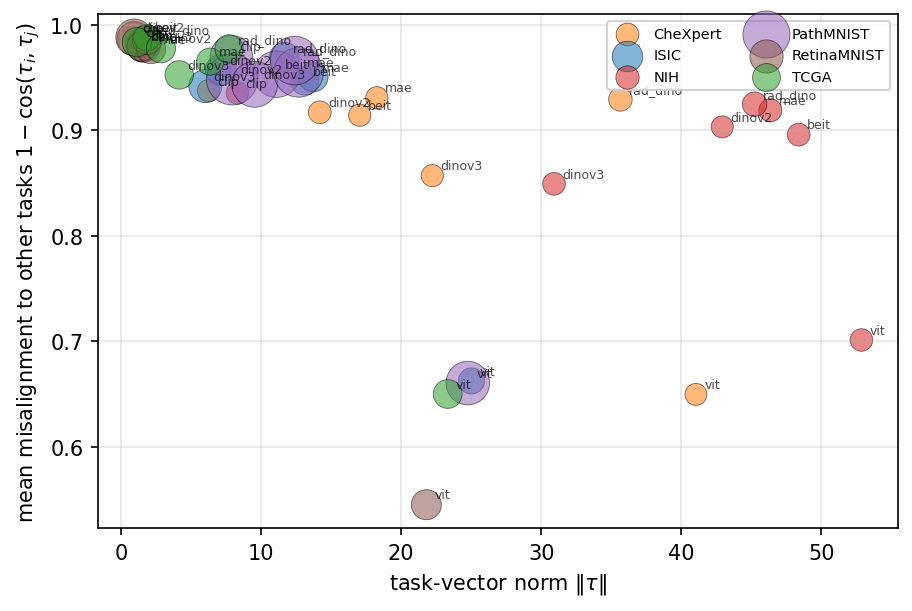
\includegraphics[width=0.6\linewidth]{norm_vs_cos_scatter.png}
\caption{All 28 (backbone, dataset) cells in the $(\|\tau\|, 1{-}\cos)$ plane, averaged across the 3 seeds. Color encodes dataset. Marker size $\propto$ mean forgetting across 8 merging methods.}
\label{fig:norm_vs_cos}
\end{figure}

\subsection{Specialists, MTL, and the merge ceiling}
\label{sec:mtl-merging}

\begin{center}
\scriptsize
\begin{tabular}{lcccc}
\toprule
       & ISIC & CheXpert & TCGA & NIH \\
\midrule
Best specialist & 0.739 (DINOv3) & 0.813 (RAD) & 0.837 (CLIP) & 0.872 (RAD) \\
Best merged     & 0.739 (CLIP/F) & \textbf{0.823} (RAD/DT) & 0.745 (CLIP/PCB) & \textbf{0.874} (RAD/DT) \\
Best MTL        & 0.703 (CLIP)   & 0.813 (RAD) & \textbf{0.794} (ViT) & 0.873 (RAD) \\
\midrule
Gap (merge--spec) & $0.000$ & $+0.010$ & $\mathbf{-0.092}$ & $+0.002$ \\
Gap (MTL--spec)   & $-0.036$ & $0.000$ & $\mathbf{-0.043}$ & $+0.001$ \\
\bottomrule
\end{tabular}
\end{center}

\noindent All values are 3-seed averaged and restricted to the 4 original backbones (CLIP, ViT, DINOv3, RAD-DINO) where the MTL baseline was run. On the radiology cluster (CheXpert and NIH), all three approaches are within a percentage point of each other and any of them is a reasonable deployment choice. The two histopathology + dermoscopy datasets break that symmetry in opposite directions. On TCGA, merging falls $9.2$ points short of the specialist while MTL recovers about half of that loss ($4.3$ points short); on ISIC the pattern flips, with merging matching the specialist while MTL falls $3.6$ points short, likely because round-robin sampling under-weights ISIC (the smallest dataset at $\approx 2{,}000$ training images) relative to the radiology datasets ($>100{,}000$ each). The net cross-method picture is two complementary failure modes: weight-space averaging hurts the dataset whose task vectors are most geometrically extreme (TCGA), and joint training hurts the dataset most starved of gradient signal under uniform sampling (ISIC). Adding the three newer backbones (DINOv2, MAE, BEiT) to the merge side raises the best-merge numbers modestly on ISIC and NIH but does not change the qualitative picture (Appendix~A).

\subsection{No merging method dominates}
\label{sec:method-ranking}

Within each dataset, the best-performing merging method varies. Fisher-weighted merging wins ISIC, DARE-TIES wins the radiology cluster (CheXpert and NIH), and PCB-Merging wins lung histopathology (TCGA), consistent with the methods literature \cite{yadav2023ties,yu2024language,du2024parametercompetitionbalancingmodel}. The lift from picking the best method per cell over a fixed default ($\alpha=0.3$ Task Arithmetic) is comparable to the within-dataset variance, so per-cell hyperparameter search is necessary in practice. We treat method ranking as a routine empirical exercise rather than a contribution.

\subsection{Cosine geometry as a cross-architecture predictor}
\label{sec:predictability}

A natural question, given the strong per-dataset structure, is whether task-vector cosine similarity carries cross-architecture signal about which (backbone, dataset, method) cells will collapse. We test this under leave-one-backbone-out (LOBO) cross-validation across all 7 backbones. Dataset+method dummies alone deliver a moderate predictor (median LOBO $R^2 = 0.36$ across seeds), substantially weaker than the corresponding value on a wider-spread cluster grid because the 4-dataset spread is itself narrower. Adding the cosine feature contributes essentially nothing on average (median $\Delta R^2 = -0.014$), and per-seed permutation tests show small lifts that flip sign across seeds (per-seed details in Appendix~B). The within-grid signal is real, however: pooled across the 28 (backbone, dataset) cells, $1{-}\cos$ tracks mean forgetting at Spearman $\rho \approx 0.66$. Cosine geometry is informative within a backbone family but does not behave as a generalizable cross-backbone predictor.

\begin{figure}[h]
\centering
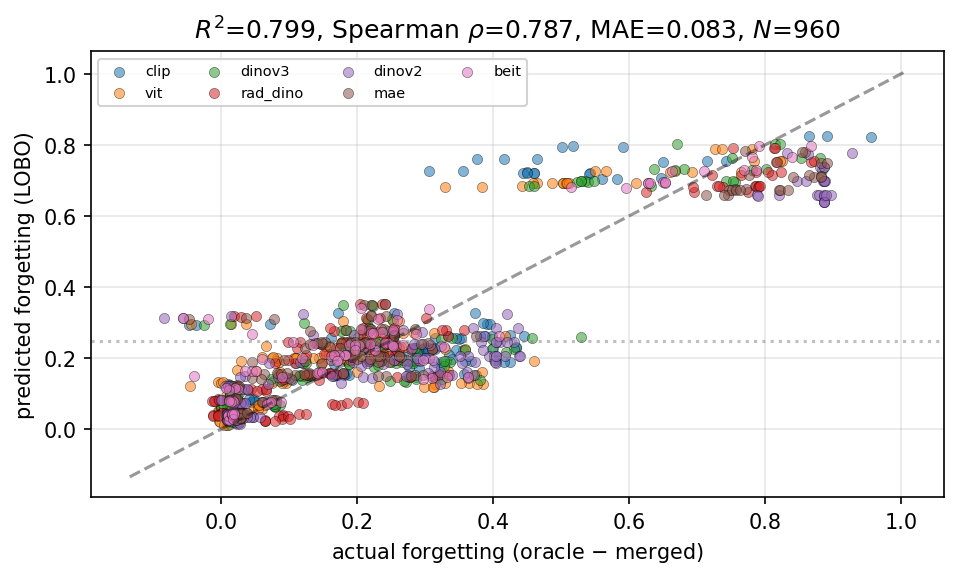
\includegraphics[width=0.7\linewidth]{lobo_predictions.png}
\caption{LOBO predictions vs.\ observed forgetting from cosine + dataset/method dummies, pooled across all 3 seeds and 7 backbones. Color encodes held-out backbone. Dashed line is $y=x$ and dotted line is the global mean.}
\label{fig:lobo_predictions}
\end{figure}

Cosine is still useful operationally even without forecasting power. Routing the bottom-half-cosine cells to the specialist oracle instead of running a merge sweep gives mean primary metric $0.78$ vs full-merge $0.76$ on the 28-cell best-merge grid at 50\% compute saved (Appendix~B). The lift is modest in the 4-dataset regime because no cell collapses to near-chance, but the policy still pays for itself because the hardest cells (low-cosine, high-forgetting) are also the most expensive to merge-sweep.

\section{Discussion}

Three approaches are on the table for serving multiple medical-imaging tasks from a shared ViT encoder: per-task specialists with a router, weight-space merging, and MTL. On the radiology cluster (CheXpert + NIH) all three sit within a percentage point of each other, so the choice is driven by deployment constraints (does training data ever live in one place? can the head architecture be jointly trained?) rather than accuracy. On the remaining two datasets, merging and MTL fail in opposite directions, and the natural interpretation is structural. TCGA's binary lung-histopathology task vectors are large and disjoint from any of our backbones' pretraining distributions (visible in the right tail of Figure~\ref{fig:norm_vs_cos}); fine-tuning produces a narrow, dataset-specific configuration that weight-space averaging perturbs heavily, while joint training keeps the encoder in a region where the TCGA-aligned and radiology/dermoscopy-aligned features can coexist. ISIC pushes the opposite way: its small training set is easy for merging to retain (the specialist's task vector is modest in norm and the dataset doesn't dominate the average), but starved of gradient signal under MTL's round-robin sampling. Neither failure is irreducible: a properly-tuned MTL with dataset-weighted sampling would likely close the ISIC gap, and merging methods with explicit interference control (PCB, DARE-TIES) already close part of the TCGA gap. Cosine geometry, despite not generalizing as a cross-backbone predictor, is useful as a compute-triage signal because the cells with lowest task-vector cosine are also the cells most likely to collapse, so routing them to specialists captures most of the lost accuracy at 50\% compute saved.

\section{Limitations and Future Work}

The backbone zoo of $N = 7$ is small, and the jackknife SE on $\Delta R^2$ spans a wide range across seeds, dominated by single-backbone leverage. The zoo is also heterogeneous in scale, with DINOv3 at ViT-S/16 ($\sim$22M params) and the other six at ViT-B/16 ($\sim$86M), so cross-backbone comparisons mix scale with pretraining-objective differences. MTL was run only on the original 4 backbones (CLIP, ViT, DINOv3, RAD-DINO) and used a default specialist optimizer with 4 epochs without further tuning; a properly-tuned MTL baseline could change the merge-vs-MTL deltas, especially on ISIC where round-robin sampling under-serves the smallest dataset. Some 2024-era methods (RegMean, AdaMerging, Localize-and-Stitch) are not benchmarked, and cosine requires fine-tuned specialists up front, so the predictor is not free. We deliberately restrict the submission to the 4 datasets where the MTL baseline exists; preliminary results on two additional MedMNIST subsets (PathMNIST colon histopathology, RetinaMNIST fundus) suggest that merging can fail catastrophically on tasks visually disjoint from any pretraining distribution, and we defer that analysis until MTL coverage is extended to those datasets. Scope is restricted to ViT backbones, $224\times224$ images, classification only, and one-shot rather than continual merging. Several of our datasets are themselves multi-source (TCGA, ISIC), so the cross-domain shift we study is overlaid on uncontrolled within-dataset institutional and scanner shift, which we do not disentangle.

\section{Contributions and Code}

This is a solo project. Sonnet Xu performed all design, implementation, cluster experiments, analysis, and writing. Code, configs, and analysis scripts are at \url{https://github.com/sonnetx/med-merge}.

\newpage
\bibliographystyle{ACM-Reference-Format}
\bibliography{reference}

\newpage
\appendix

\section{Specialist baselines (full grid)}

Per-(backbone, dataset) specialist primary metric, averaged across all 3 seeds. The primary metric is balanced accuracy on ISIC, macro-AUROC on CheXpert and NIH, and AUROC on TCGA.

\begin{center}
\small
\begin{tabular}{lcccc}
\toprule
Backbone & ISIC & CheXpert & TCGA & NIH \\
\midrule
CLIP     & 0.735 & 0.808 & 0.837 & 0.867 \\
ViT      & 0.725 & 0.803 & 0.800 & 0.865 \\
DINOv3   & 0.739 & 0.809 & 0.813 & 0.869 \\
RAD-DINO & 0.675 & 0.813 & 0.759 & 0.872 \\
DINOv2   & 0.684 & 0.797 & 0.735 & 0.854 \\
MAE      & 0.669 & 0.772 & 0.819 & 0.838 \\
BEiT     & 0.746 & 0.795 & 0.644 & 0.868 \\
\bottomrule
\end{tabular}
\end{center}

The four datasets sit in a relatively narrow specialist-accuracy band ($0.64$--$0.87$), so absolute forgetting in \S\ref{sec:dataset-clusters} maps cleanly to relative loss without the interpretation hazards that arise when specialists themselves are weak. RAD-DINO leads on the two radiology datasets, as expected from its in-domain pretraining; the natural-image backbones are within 1--2 points on CheXpert and NIH.

\section{LOBO predictor details and screening ablation}

Per-seed LOBO regression results for the cosine + dataset/method-dummies predictor of merge forgetting on the 4-dataset, 7-backbone grid. The columns report the dummies-only $R^2$, the +cosine $R^2$, their difference, the corresponding difference in Spearman $\rho$, and the two-sided $p$-value from a $1000$-permutation test on the cosine column.

\begin{center}
\small
\begin{tabular}{lccccc}
\toprule
seed & dummies $R^2$ & +cosine $R^2$ & $\Delta R^2$ & $\Delta \rho$ & perm.\ $p$ \\
\midrule
42  & $0.35$ & $0.34$ & $-0.014$ & $-0.002$ & $0.061$ \\
123 & $0.36$ & $0.34$ & $-0.019$ & $-0.009$ & $0.015$ \\
456 & $0.39$ & $0.38$ & $-0.005$ & $+0.011$ & $0.555$ \\
\midrule
median & $\mathbf{0.36}$ & $0.34$ & $\mathbf{-0.014}$ & $-0.002$ & --- \\
\bottomrule
\end{tabular}
\end{center}

\noindent\textbf{Cosine-screening ablation.} On the 28-cell best-merge grid (7 backbones $\times$ 4 datasets, seed-averaged), threshold cosine at the per-cell median and below threshold fall back to the specialist oracle instead of running the merge sweep. The achieved mean primary metric is $0.78$ with this 50\%-compute-saved policy, versus a full-merge baseline of $0.76$. The lift is small in absolute terms because no cell in the 4-dataset regime collapses to near-chance, but the policy is essentially free.

\section{Fisher-wins-ISIC validation}

Fisher matrices computed on small validation sets have large magnitude, so Fisher-weighted merging concentrates on the dataset with the smallest validation set. We verify directly. ISIC's per-dataset Fisher magnitude (sum of $|F_d|$ over parameters) is between $\mathbf{120\times}$ (RAD-DINO) and $\mathbf{1000\times}$ (DINOv3) larger than the radiology datasets'. Practitioners should normalize Fisher matrices by validation-set size before merging in heterogeneous-data regimes. (Note that the Fisher diagonal computed for TCGA is exactly zero in our cache, a binary-classification edge case, so the Fisher merge on TCGA behaves as the Fisher-weighted average of the non-TCGA task vectors only.)

\end{document}
